\documentclass[tikz,border=2pt]{standalone}
\usepackage{amsmath}
\usepackage{pgfplots}
\pgfplotsset{compat=1.18}
\usetikzlibrary{arrows.meta}
\begin{document}
% Example 1: quadrilateral V with Ext(V)={(0,0),(3,0),(2,3),(0,4)}; supporting line H: x1+2x2=8 meets V in the edge
% from (0,4) to (2,3), whose extreme points are the extreme points of V on H.
% Example 4: square [0,2]x[0,2] cut by x2=1 (not supporting): the end points (0,1),(2,1) of the cut are not extreme in V.
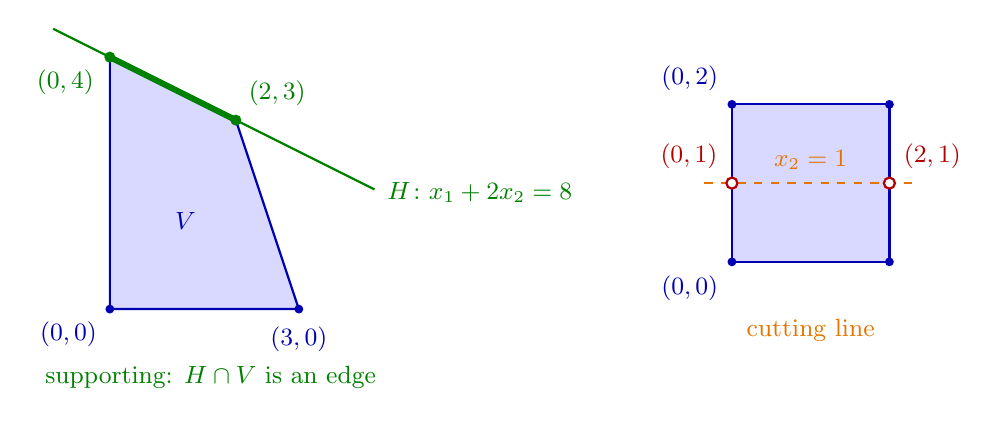
\begin{tikzpicture}[font=\small, >={Latex[length=2mm]}]
  \begin{scope}[x=0.8cm, y=0.8cm]
    \fill[blue!15] (0,0) -- (3,0) -- (2,3) -- (0,4) -- cycle;
    \draw[blue!70!black, thick] (0,0) -- (3,0) -- (2,3) -- (0,4) -- cycle;
    \node[blue!70!black] at (1.2,1.4) {$V$};
    \draw[green!50!black, thick] (-0.9,4.45) -- (4.2,1.9);
    \draw[green!50!black, line width=2.2pt] (0,4) -- (2,3);
    \fill[blue!70!black] (0,0) circle (1.6pt) (3,0) circle (1.6pt);
    \fill[green!50!black] (0,4) circle (2pt) (2,3) circle (2pt);
    \node[blue!70!black, anchor=north east] at (-0.05,-0.05) {$(0,0)$};
    \node[blue!70!black, anchor=north] at (3,-0.12) {$(3,0)$};
    \node[green!50!black, anchor=north east] at (-0.1,3.95) {$(0,4)$};
    \node[green!50!black, anchor=south west] at (2.05,3.08) {$(2,3)$};
    \node[green!50!black, anchor=west] at (4.25,1.85) {$H\colon x_1+2x_2=8$};
    \node[green!50!black, anchor=north] at (1.6,-0.75) {supporting: $H\cap V$ is an edge};
  \end{scope}
  \begin{scope}[xshift=7.9cm, yshift=0.6cm, x=1cm, y=1cm]
    \fill[blue!15] (0,0) rectangle (2,2);
    \draw[blue!70!black, thick] (0,0) rectangle (2,2);
    \fill[blue!70!black] (0,0) circle (1.6pt) (2,0) circle (1.6pt) (0,2) circle (1.6pt) (2,2) circle (1.6pt);
    \node[blue!70!black, anchor=north east] at (-0.05,-0.05) {$(0,0)$};
    \node[blue!70!black, anchor=south east] at (-0.05,2.05) {$(0,2)$};
    \draw[orange!90!black, thick, dashed] (-0.35,1) -- (2.35,1);
    \node[orange!90!black, anchor=south] at (1,1.05) {$x_2=1$};
    \draw[red!70!black, thick, fill=white] (0,1) circle (2pt) (2,1) circle (2pt);
    \node[red!70!black, anchor=south east] at (-0.06,1.06) {$(0,1)$};
    \node[red!70!black, anchor=south west] at (2.06,1.06) {$(2,1)$};
    \node[orange!90!black, anchor=north] at (1,-0.6) {cutting line};
  \end{scope}
\end{tikzpicture}
\end{document}
